% !TEX root = ./paper.tex
% Background and motivation

%TODO
%Gives an overview of \tls / \tcp and how they interact. We also need a comparison
%of QUIC and \tls/\tcp on several points that would serve as a base to explain why
%\tls 1.3's extensibility cannot compete with QUIC.
%Gives an overview of \tls / \tcp and how they interact.

\begin{figure}[!t]
  \begin{center}
    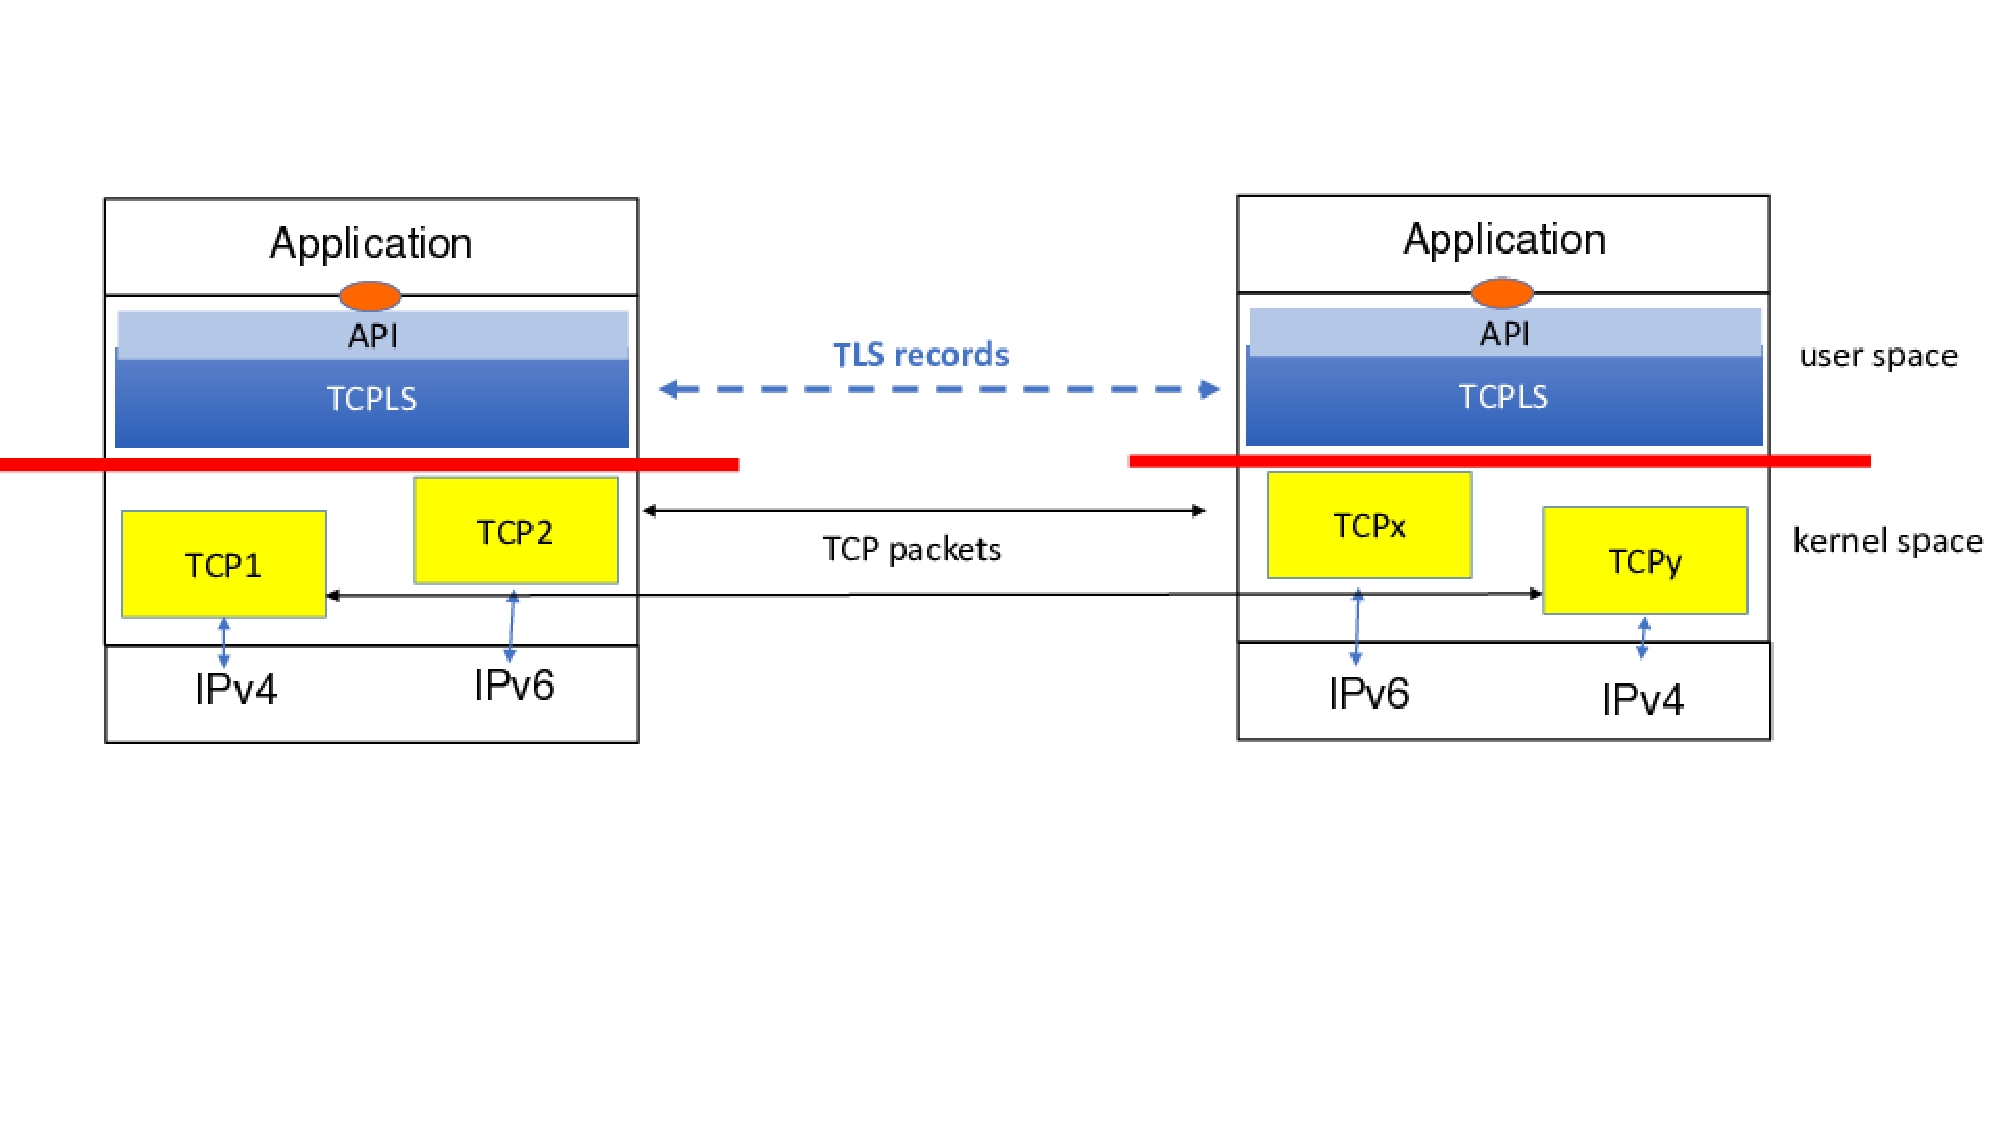
\includegraphics[width=8cm]{figures/tcpls-fig2.pdf}
  \end{center}
  \caption{\tcpls in the stack.}
  \label{fig:arch}
\end{figure}

\tcpls (illustrated in Fig.~\ref{fig:arch}) offers a cross-layer interface to \tls and \tcp with the motivation to do more than securing the transport layer. Merging the stacks benefits both protocols and the application using this new approach. First, \tcp suffers from a lack of extensibility due to size restrictions in its header and due to potential middlebox interferences~\cite{honda2011still}. \tcpls aims to solve \tcp extensibility issue in the long run by offering a secure control channel to exchange \tcp options without suffering from middlebox interferences and size restrictions in \tcp headers. Second, \tls does not have a clear view of the transport protocol, and offering one with \tcpls brings opportunity for performance improvement (e.g., avoiding records fragmentation with dynamic receive buffer auto-tuning and/or with dynamic control of the record length), and for connection reliability (e.g., failover).  Third, applications are becoming more complex, which appeals to exposing transport-level functionalities and letting them tune the underlying transport to their use case. Essentially, this last motivation discusses a novel manner to expose transport-level functionalities that are encrypted, authenticated, reliable, extensible, and adapted to complex application-level requirements.

\subsection{Overview}

\tcp separates control information and data by placing the control information
in the packet header and the data in the payload. This separation worked well
until middleboxes started to interfere with \tcp~\cite{10.1145/1064413.1064418,
  honda2011still, DHBVD13}.  On a fraction of Internet paths, including e.g.,
some enterprise and cellular networks, some middleboxes interfere by adding,
removing, or changing \tcp options~\cite{wang2011untold, honda2011still,
  xu2015investigating} and, in some cases, also transparently terminating \tcp
connections. These middleboxes have slowed down the evolution of \tcp in recent
years. \tcpls also uses the packet header to exchange \tcp control information,
but it leverages \tls to create a second and secure control channel. In a
nutshell, \tcpls leverages the extensibility of \tls 1.3 to place control
information such as \tcp options inside the \tls handshake messages and new \tls
records. Since this information is encrypted and authenticated, the
communicating hosts can exchange new control information without encountering
middlebox interference.
%We describe several examples of these new types of
%control information in Sec.~\ref{sec:extending} and Sec.~\ref{sec:connmigr}.

Once the \tcpls session has been established, \tcpls requires the upper layer to
open streams and attach them to the session. A stream is an independant
cryptographic context derived from the \tcpls handshake. They must be attached to a \textit{Connected} \tcp bytestream exported as a \texttt{transportid} to the application. To manipulate streams, \tcpls offers an API to open, attach
and close streams to any available \texttt{transportid} in the \textit{Connected} state, while offering the Stream as the only bytestream abstraction to the upper layer. Streams can only be attached to one \texttt{transportid}, but they can be moved, several streams can be attached to a given \texttt{transportid}, and multiple streams can be attached to multiple \texttt{transportid}s.

\tcpls can attach streams using the Secure Control Channel and send TLS records
within them in a zero-rtt fashion. That is, when the peer receives a
\texttt{STREAM\_ATTACH} message in the control channel, it has everything needed
to securly derive the right cryptographic context to process the TLS record
encryted within this stream. No round-trips are needed to attach a new stream.
Most of records encrypted with a Stream's context contain application data
transmitted by the client or the server. However, streams can also carry control
records.
%The control channel between the client and the server
%enables \tcpls to define a new bytestream abstraction and support many new
%features while benefitting from the current kernel and network optimization for
%\tcp performance.

%Applications such as HTTP/2 support multiple streams mapped to a single \tcp
%connection. However, there are situations, e.g., to prevent head-of-line
%blocking, where different streams should be mapped over other underlying \tcp
%connections. With \tcpls, the client and the server can establish different
%datastreams over a single \tcpls session, preventing \tcp's HOL. Thus, a
%\tcpls session can be composed of one or more \tcp connections similarly as a
%\mptcp connection gathers subflows.

To support data from a given datastream to be exchanged over several \tcp
connections, \tcpls includes its sequence numbers when the multipath aggregation
mode is activated. A client and server can also enable acknowledgments. Thanks
to these \tcpls acknowledgments, a \tcpls session can react to the failure of
the underlying \tcp connection by reestablishing a new \tcp connection to
continue the data transfer and replay the records that have been lost.

A \tcp connection ends with the exchange of \fin or \rst packets. However, some
middleboxes force the termination of \tcp connections by sending \rst
packets~\cite{rfc3360,weaver2009detecting}. \tcpls can preserve established
connections by automatically restarting the underlying \tcp connection upon
reception of a spurious reset. \tcpls defines the connection termination at the
stream level: closing the last stream attached to a \tcp connection allows
clients and servers to securely terminate the \tcpls session.

That is, with the Secure Control Channel, we offer a flexible bytestream
abstraction to the upper layer that supports various new features such as
Streams, Connection reliability, various secure multipath modes, secure
connection closing,  encrypted \tcp options and benefit from \tcp's state of performance and \tls's state of deployment.

%Todo explain that the transport abstraction level failed to offera versatile
%usage
%of the transport layer, and explain how a session layer can repair the
%abstraction
%Besides, with our design of \tcp extensibility
%within \texttt{\tcpLS}, applications would be able to tune \tcp on a connection basis,
%using existing options or any future option without middlebox interferences. As
%a matter of example, our \texttt{\tcpLS} implementation supports several
%\tcp options that can difficulty live at the \tcp layer
%(e.g., Joining a Multipath connection, injecting eBPF bytecode to the kernel's
%peer to tune \tcp). With \texttt{TCPLS}, we show how to solve several of these
%existing problem.

%Finally, \texttt{\tcpLS}'s control channel is expected to offer extensibility
%without middlebox interference and with protocol message indistinguishability
%from the network to avoid fingerprinting of the client stack. Our objective is
%to design a versatile \tcp extensibility mechanism that would allow to set
%options, exchange eBPF bytecode~\cite{de2019pluginizing} to tune the peer's kernel and implement new
%session behaviours.
